\documentclass[12pt]{article}
\usepackage[utf8]{inputenc}
\usepackage[spanish]{babel}
\usepackage{geometry}
\usepackage{graphicx}
\usepackage{fancyhdr}
\usepackage{hyperref}

% --- CONFIGURACIÓN DE LA PÁGINA ---
% Márgenes
\geometry{a4paper, margin=2.5cm}

% Encabezado y pie de página personalizados
\pagestyle{fancy}
\fancyhf{} % Limpia los campos de encabezado y pie
\lhead{Bases de Datos a Gran Escala} % Encabezado izquierdo
\rhead{Práctica 4: Consultas OLTP}   % Encabezado derecho
\cfoot{\thepage}                     % Pie de página centrado (número de página)

% --- DOCUMENTO ---
\begin{document}

% --- PORTADA ---
\begin{titlepage}
    \centering
    \vspace*{1cm}
    \Huge
    \textbf{Práctica 4: Consultas OLTP en PostgreSQL}
    
    \vspace{1.5cm}
    \Large
    Bases de Datos a Gran Escala
    
    \vspace{2.5cm}
    
    \Large
    \textbf{Integrantes del equipo 13:}
    \vspace{0.5cm}
    
    % AÑADE AQUÍ LOS NOMBRES DE LOS INTEGRANTES
    Andres Lopez Gonzalez \\
    Carlos Fabian Esteva Gallegos
    
    \vfill % Empuja el contenido hacia abajo
    
    \large
    % \today genera la fecha actual automáticamente
    \today
    
\end{titlepage}


% --- OBJETIVO ---
\section*{Objetivo}
Realizar consultas en SQL a las bases de datos de los sistemas de \textbf{Reclusorios} y \textbf{Pacientes} en una base de datos PostgreSQL, aplicando diversas cláusulas y uniones para la extracción de información específica.

\rule{\linewidth}{0.5mm}


% --- ACTIVIDAD 1 ---
\section{Actividad 1: Carga de Datos}
Se realiza la carga de 10 registros en las entidades fuertes y los correspondientes en las entidades débiles para cada base de datos, respetando las restricciones de integridad y formato de llaves primarias.

\subsection{Carga en Base de Datos Reclusorios\_013}
\vspace{5mm}
\noindent\rule{\linewidth}{0.4pt}
\begin{figure}[h]
    \centering
    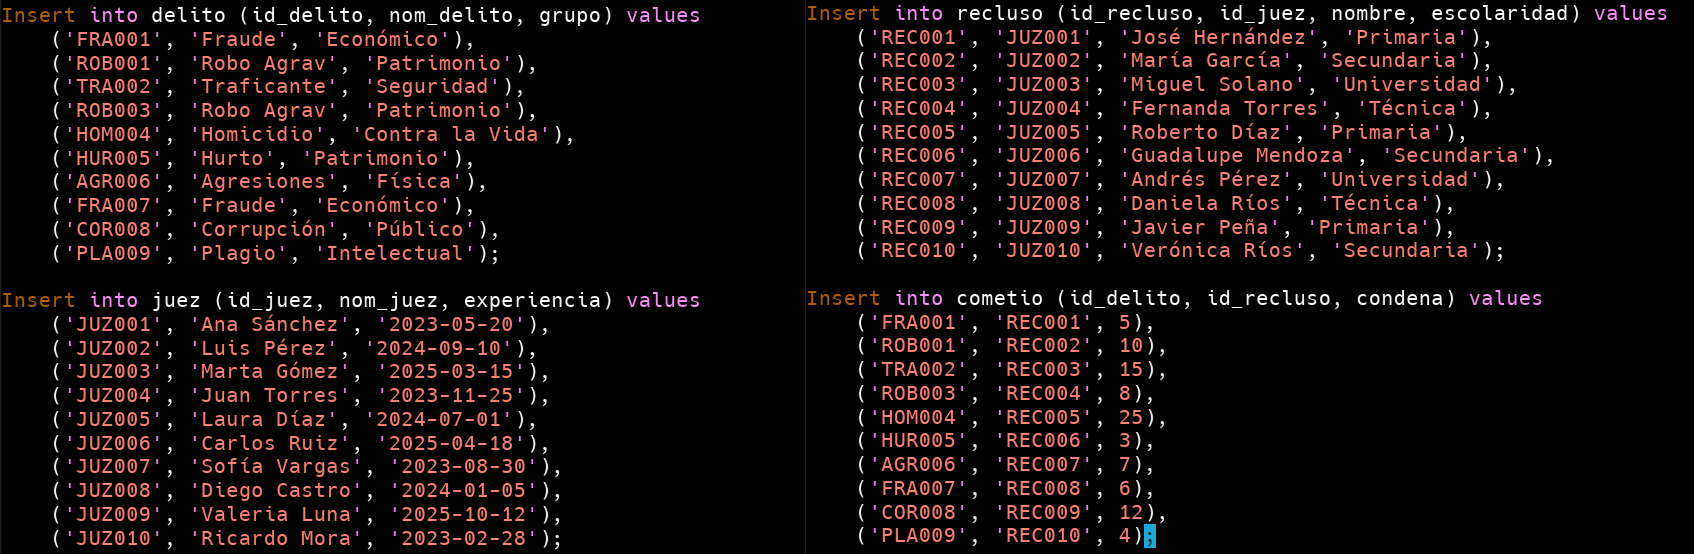
\includegraphics[width=1\linewidth]{Captura de los comandos 'INSERT INTO...' para las tablas de Reclusorios.png}
    \caption{Captura de los comandos 'INSERT INTO...' para las tablas de Reclusorios.}
    \label{fig:placeholder}
\end{figure}\\
\noindent\rule{\linewidth}{0.4pt}
\vspace{5mm}


\subsection{Carga en Base de Datos Pacientes\_013}
\vspace{5mm}
\noindent\rule{\linewidth}{0.4pt}
\begin{figure}[h]
    \centering
    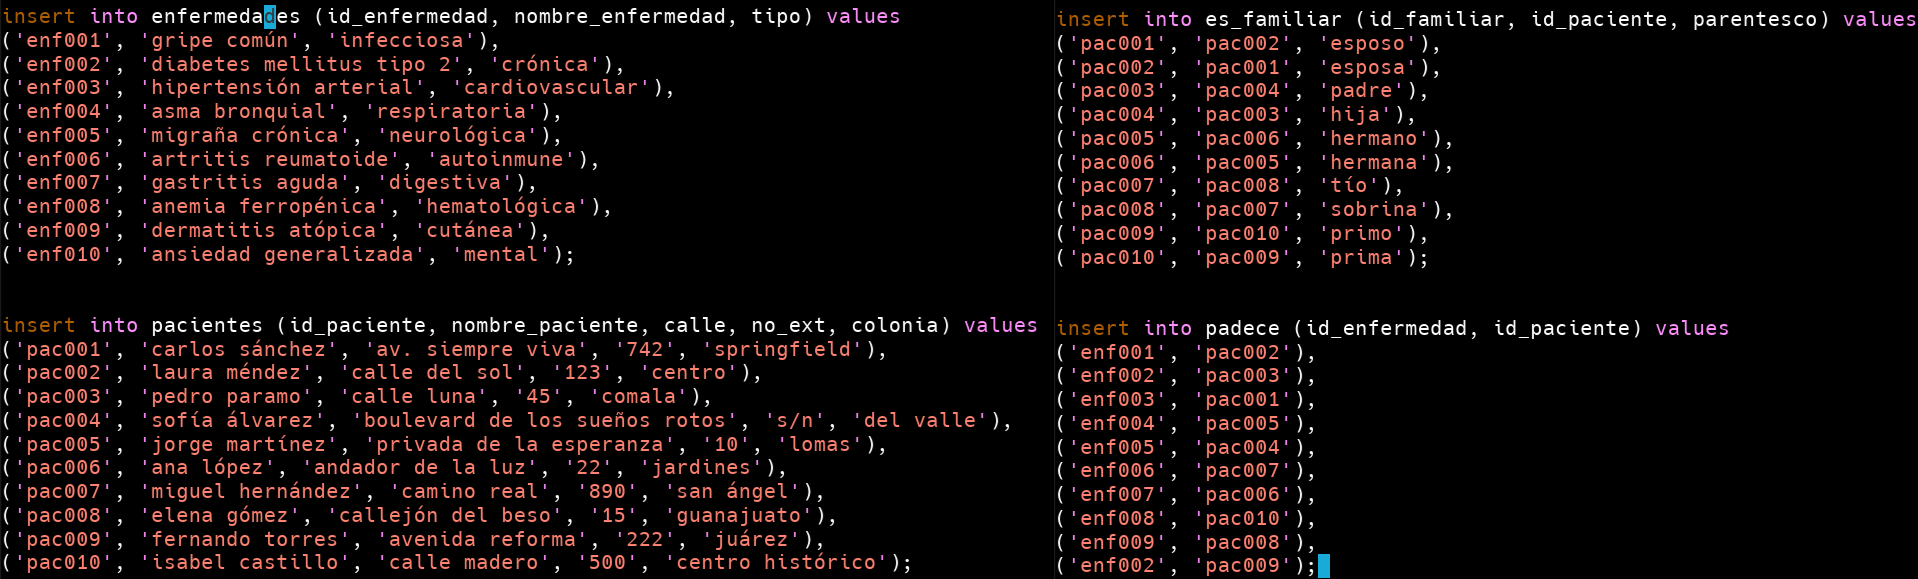
\includegraphics[width=1\linewidth]{Captura de los comandos 'INSERT INTO...' para las tablas de Pacientes..png}
    \caption{Captura de los comandos 'INSERT INTO...' para las tablas de Pacientes.}
    \label{fig:placeholder}
\end{figure}\\
\noindent\rule{\linewidth}{0.4pt}
\vspace{5mm}

\newpage
\rule{\linewidth}{0.5mm}


% --- ACTIVIDAD 2 ---
\section{Actividad 2: Verificación de Datos}
Se ejecutan consultas generales para verificar que todos los datos de la Actividad 1 fueron insertados correctamente en todas las tablas de ambas bases de datos.

\subsection{Verificación en Reclusorios\_013}
\vspace{5mm}
\noindent\rule{\linewidth}{0.4pt}
\begin{figure}[h]
    \centering
    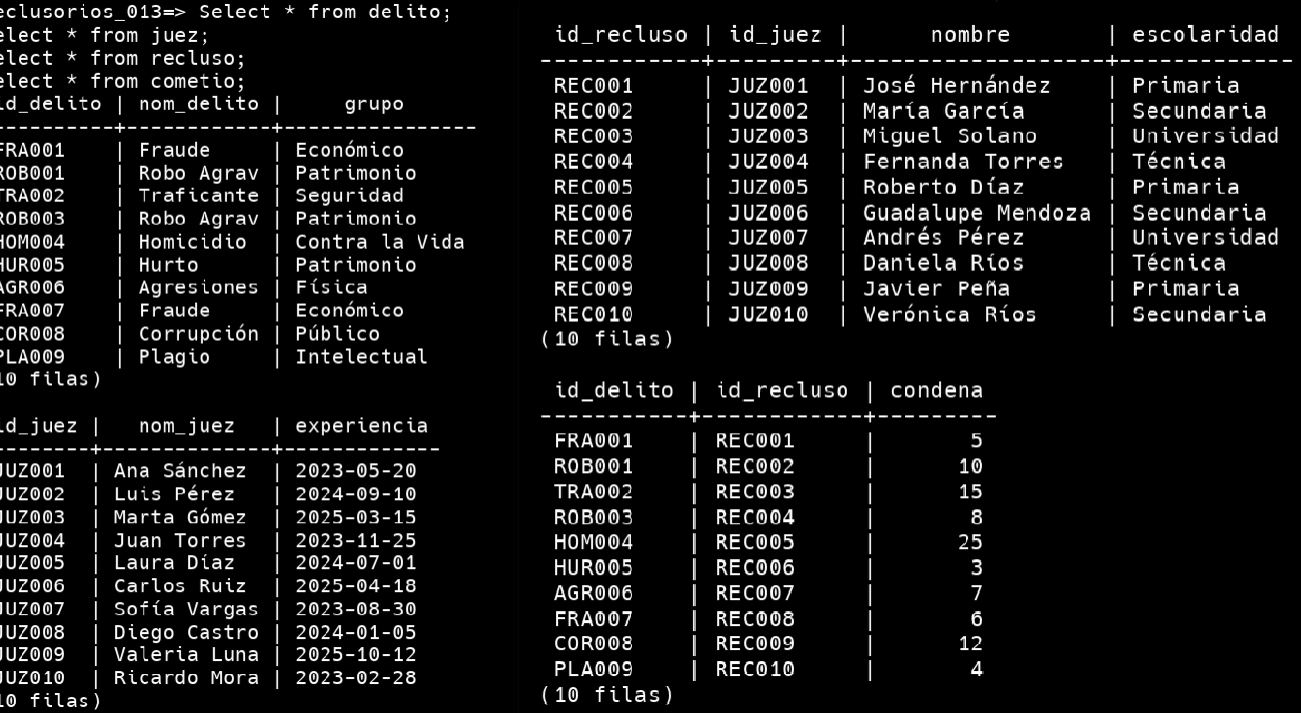
\includegraphics[width=1\linewidth]{Consulta de todos los registros en las tablas de Reclusorios.png}
    \caption{Consulta de todos los registros en las tablas de Reclusorios}
    \label{fig:placeholder}
\end{figure}\\
\noindent\rule{\linewidth}{0.4pt}
\vspace{5mm}

\subsection{Verificación en Pacientes\_013}
\vspace{5mm}
\noindent\rule{\linewidth}{0.4pt}
\begin{figure}[h]
    \centering
    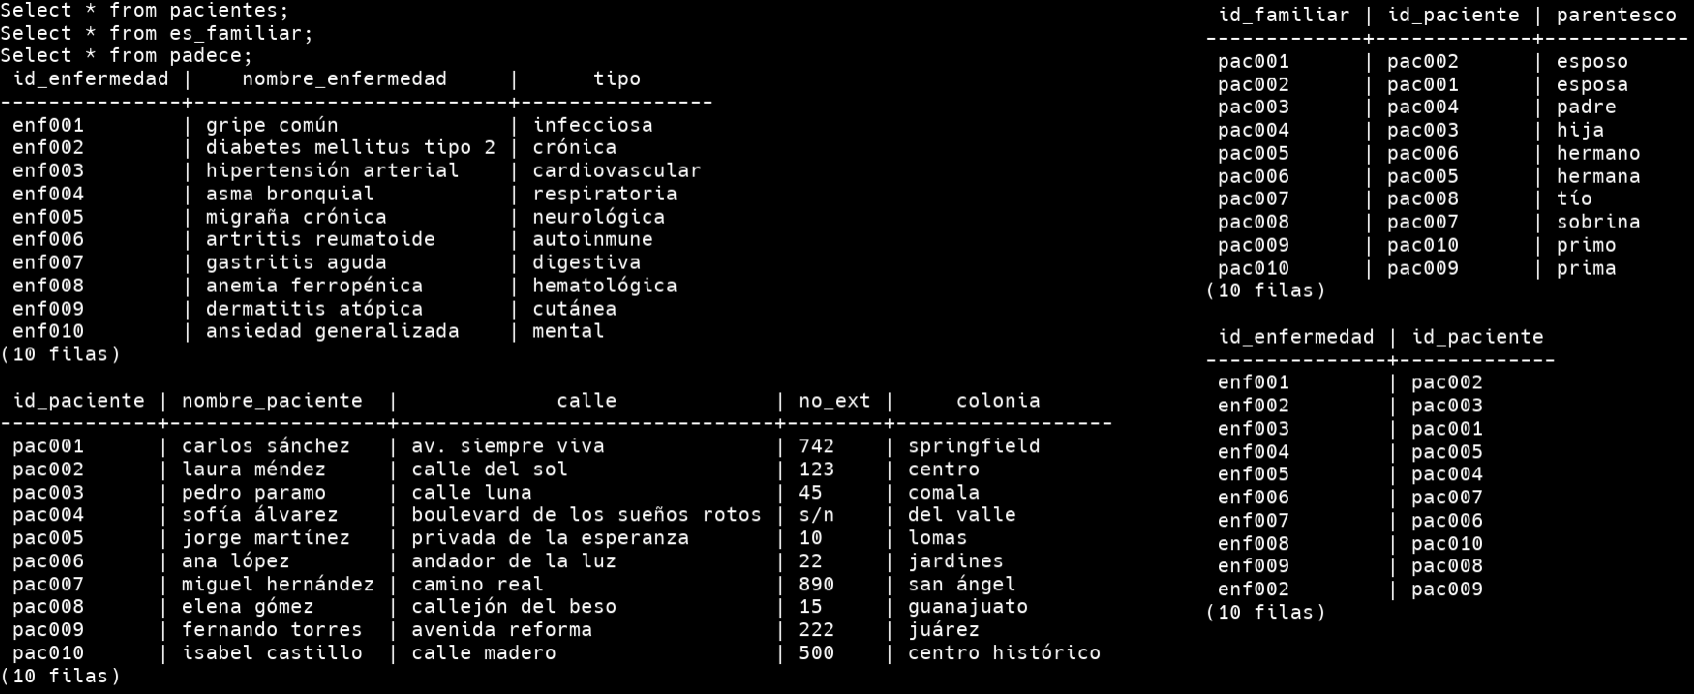
\includegraphics[width=1\linewidth]{Consulta de todos los registros en las tablas de Pacientes.png}
    \caption{Consulta de todos los registros en las tablas de Pacientes}
    \label{fig:placeholder}
\end{figure}\\
\noindent\rule{\linewidth}{0.4pt}
\vspace{5mm}

\rule{\linewidth}{0.5mm}


% --- ACTIVIDAD 3 ---
\section{Actividad 3: Consultas al Sistema Reclusorios\_013}
A continuación se presentan las consultas específicas realizadas al sistema de Reclusorios.

\subsection{Consulta 3.1: Juez y condena de un recluso}
\vspace{5mm}
\begin{figure}[h]
    \centering
    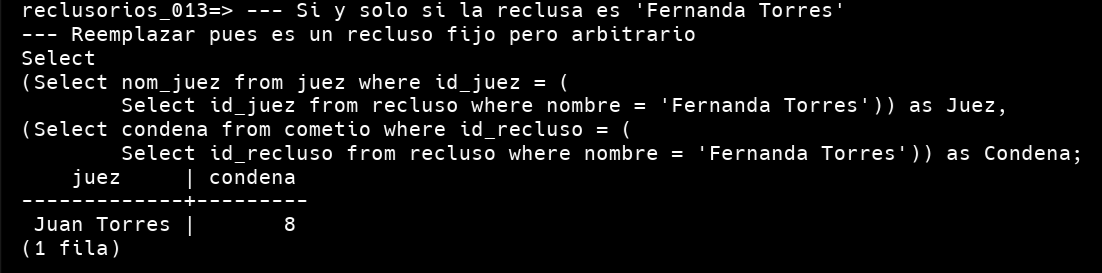
\includegraphics[width=0.75\linewidth]{r1.png}
    \label{fig:placeholder}
\end{figure}
\vspace{5mm}

\subsection{Consulta 3.2: Reclusos y promedio de condena por juez}
\textit{ }
\begin{figure}[h]
    \centering
    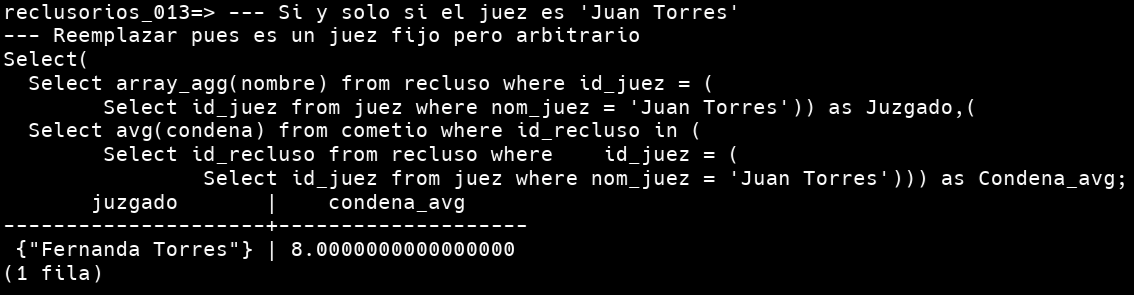
\includegraphics[width=0.75\linewidth]{r2.png}
    \label{fig:placeholder}
\end{figure}
\vspace{5mm}

\subsection{Consulta 3.3: Número de reclusos por delito}
\vspace{5mm}
\begin{figure}[h]
    \centering
    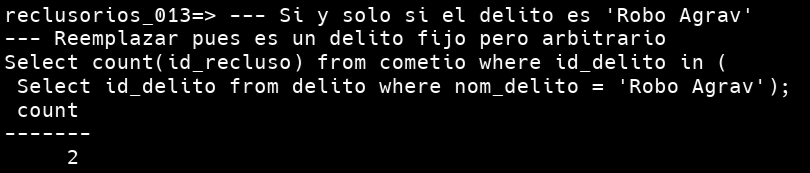
\includegraphics[width=0.75\linewidth]{r3.png}
    \label{fig:placeholder}
\end{figure}
\vspace{5mm}

\subsection{Consulta 3.4: Reclusos por número de días de condena}
\vspace{5mm}
\begin{figure}[h]
    \centering
    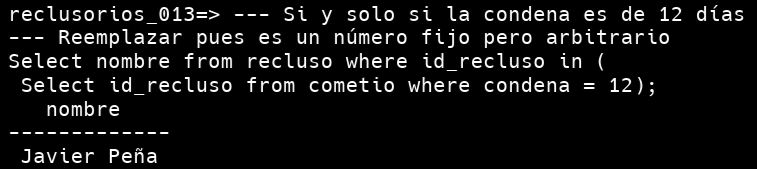
\includegraphics[width=0.75\linewidth]{r4.png}
    \label{fig:placeholder}
\end{figure}
\vspace{5mm}

\newpage
\rule{\linewidth}{0.5mm}


% --- ACTIVIDAD 4 ---
\section{Actividad 4: Consultas al Sistema Pacientes\_013}
Consultas específicas realizadas a la base de datos de Pacientes.

\subsection{Consulta 4.1: Enfermedades de un paciente}
\vspace{5mm}
\begin{figure}[h]
    \centering
    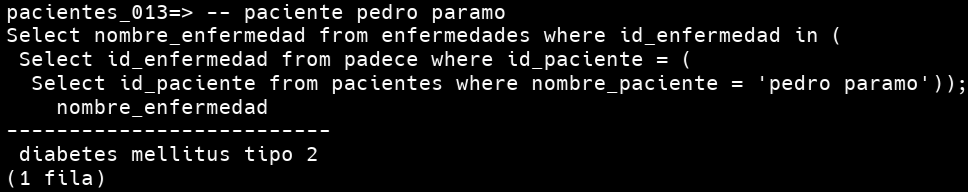
\includegraphics[width=0.75\linewidth]{p1.png}
    \label{fig:placeholder}
\end{figure}
\vspace{5mm}

\subsection{Consulta 4.2: Pacientes con una enfermedad}
\vspace{5mm}
\begin{figure}[h]
    \centering
    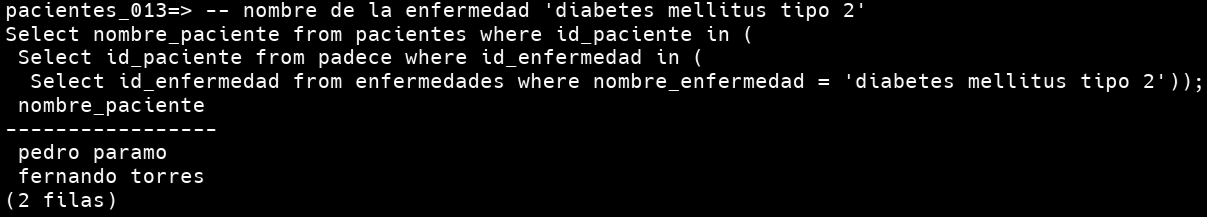
\includegraphics[width=0.75\linewidth]{p2.png}
    \label{fig:placeholder}
\end{figure}
\vspace{5mm}

\subsection{Consulta 4.3: Pacientes cuyos padres padecieron una enfermedad}
\vspace{5mm}
\begin{figure}[h]
    \centering
    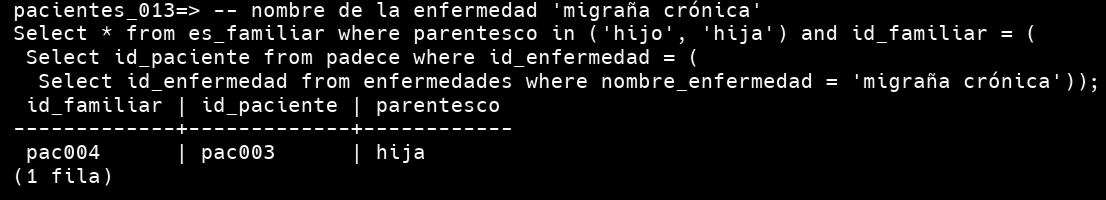
\includegraphics[width=0.75\linewidth]{p3.png}
    \label{fig:placeholder}
\end{figure}
\vspace{1mm}

\subsection{Consulta 4.4: Enfermedades de hermanos y primos de un paciente}
\textit{}
\begin{figure}[h]
    \centering
    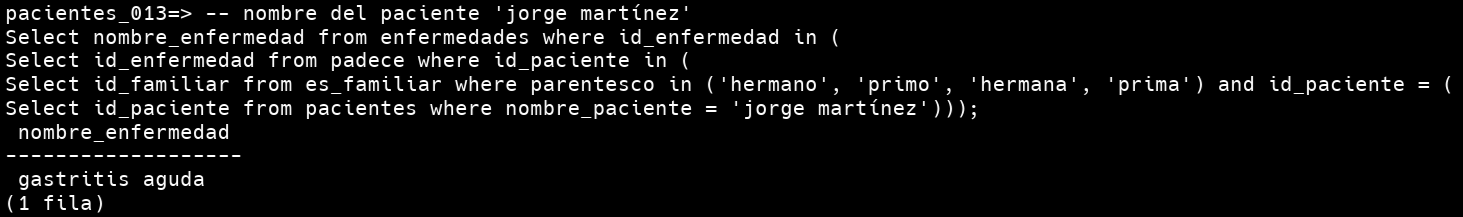
\includegraphics[width=0.95\linewidth]{p4.png}
    \label{fig:placeholder}
\end{figure}
\vspace{5mm}\\

\subsection{Consulta 4.5: Pacientes con enfermedades contagiosas}
\textit{ }
\begin{figure}[h]
    \centering
    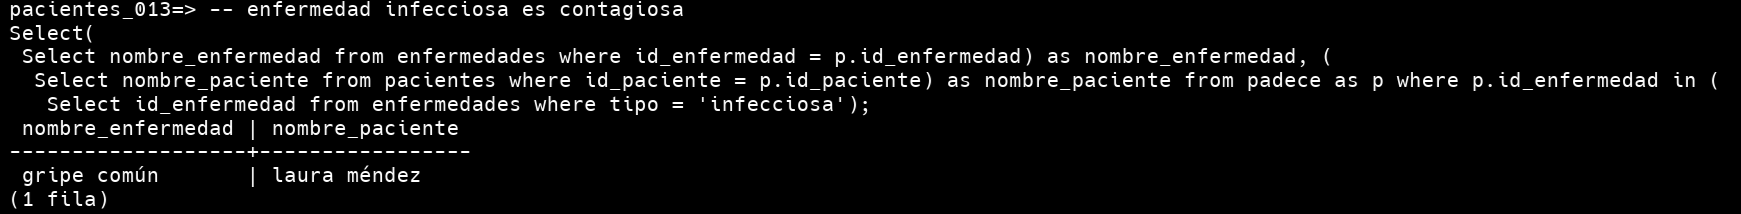
\includegraphics[width=1\linewidth]{p5.png}
    \label{fig:placeholder}
\end{figure}
\vspace{5mm}

\newpage
\rule{\linewidth}{0.5mm}


% --- ACTIVIDAD 5 ---
\section{Actividad 5: Consultas con JOINs}
Se crea la base de datos \texttt{Empleados\_Proyectos\_013} y se realizan consultas para practicar el uso de diferentes tipos de \texttt{JOIN}.

\subsection*{Creación de la BD y Carga de Datos}
\vspace{5mm}
\noindent\rule{\linewidth}{0.4pt}
\begin{figure}[h]
    \centering
    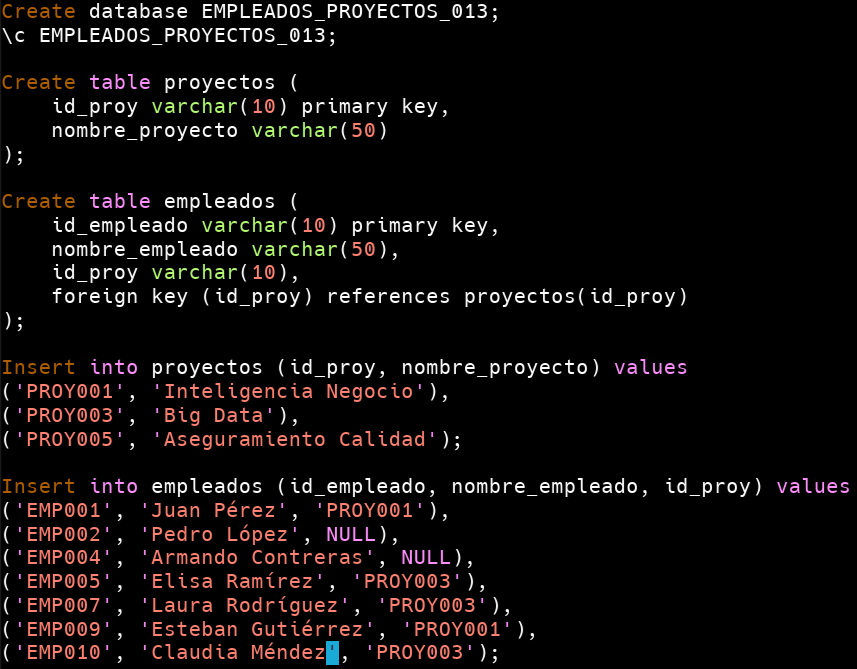
\includegraphics[width=.9\linewidth]{Vim5.png}
    \caption{Instrucciones de la actividad 5 en vim}
    \label{fig:placeholder}
\end{figure}\\
\noindent\rule{\linewidth}{0.4pt}
\vspace{5mm}

\subsection{Consulta 5.1: Empleados con proyecto asignado (INNER JOIN)}\\
\textit{ }
\begin{figure}[h]
    \centering
    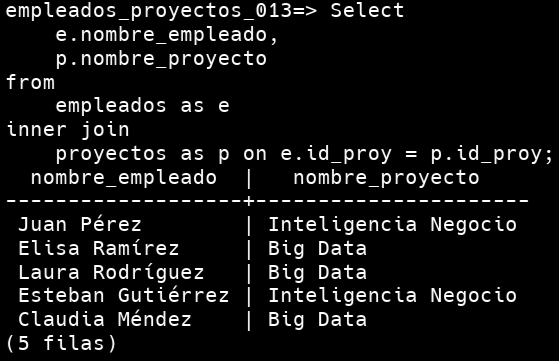
\includegraphics[width=0.75\linewidth]{inner.png}
    \label{fig:placeholder}
\end{figure}
\vspace{5mm}

\subsection{Consulta 5.2: Todos los empleados, con o sin proyecto (LEFT JOIN)}
\vspace{5mm}
\begin{figure}[h]
    \centering
    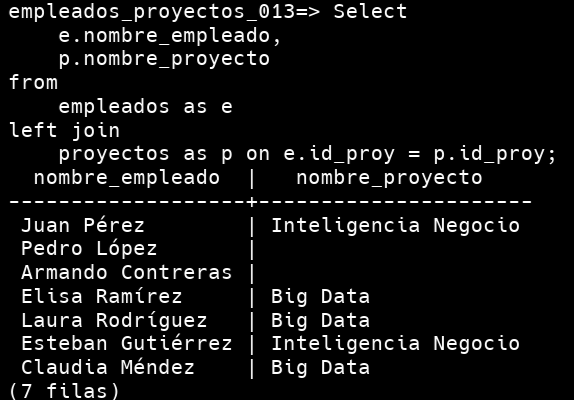
\includegraphics[width=0.75\linewidth]{left.png}
    \label{fig:placeholder}
\end{figure}
\vspace{5mm}

\subsection{Consulta 5.3: Todos los empleados y proyectos (FULL OUTER JOIN)}\\
\textit{ }
\begin{figure}[h]
    \centering
    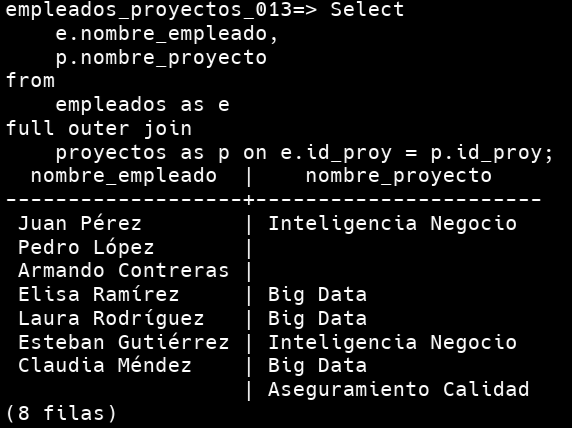
\includegraphics[width=0.75\linewidth]{full outer.png}
    \label{fig:placeholder}
\end{figure}
\vspace{5mm}

\subsection{Consulta 5.4: Empleados sin proyecto y proyectos sin empleado}\\
\textit{ }
\begin{figure}[h]
    \centering
    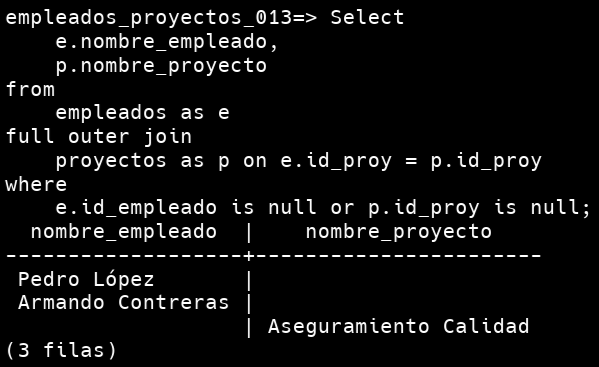
\includegraphics[width=0.75\linewidth]{sim dif join.png}
    \label{fig:placeholder}
\end{figure}
\vspace{5mm}

\subsection{Consulta 5.5: Empleados que NO tienen proyecto asignado} \\
\textit{ }
\begin{figure}[h]
    \centering
    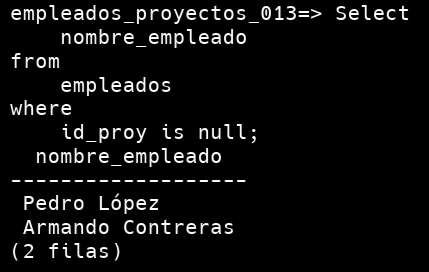
\includegraphics[width=0.75\linewidth]{noproy.png}
    \label{fig:placeholder}
\end{figure}
\vspace{5mm}\\

\subsection{Consulta 5.6: Proyectos que NO tienen empleado asignado}\\
\textit{ }
\begin{figure}[h]
    \centering
    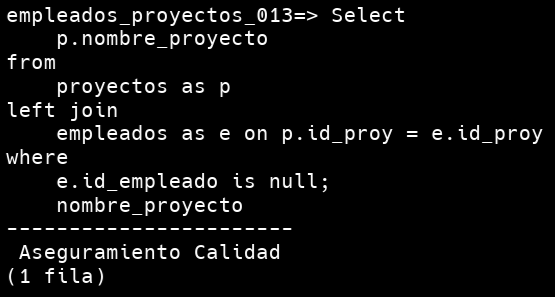
\includegraphics[width=0.75\linewidth]{noemp.png}
    \label{fig:placeholder}
\end{figure}
\vspace{5mm}

\end{document}

